\documentclass[]{article}

%%%%%%%%%%%%%%%%%  << MATLAB INCLUSION>>  %%%%%%%%%%%%%%%%%
\usepackage[numbered framed]{mcode}  % In ~/Library/texmf...
%%%%%%%%%%%%%%%%%  << MATLAB INCLUSION>>  %%%%%%%%%%%%%%%%%

%%%%%%%%%%%%%%%%%  << IMAGE INCLUSION>>  %%%%%%%%%%%%%%%%%
\usepackage{graphicx}
%%%%%%%%%%%%%%%%%  << IMAGE INCLUSION>>  %%%%%%%%%%%%%%%%%

\usepackage{cleveref}
\usepackage{amsmath}
\usepackage{color}

\begin{document}

\title{ASEN 5070-Stastistical Orbit Determination-HW 7}
\author{Zach Dischner}
\date{10-23-2012}
\maketitle


%%%%%%%%%%%%%%%%%%%%%%  << 1 >>  %%%%%%%%%%%%%%%%%%%%%%%%
\section{Problem 1} 
This assignment involved setting up the batch processor for the semester project. Basically, it was the preamble to performing a full batch/Kalman analysis on a set of observations and a model including J2 gravity effects and atmospheric drag. 

\noindent The key assumptions in building this model were:
\begin{center}
	\begin{enumerate}
		\item[$\bullet$] Three tracking stations provide instantaneous range and gran rate data
		\item[$\bullet$] The force model is to contain the effects of oblateness (J2) and atmospheric drag.
		\item[$\bullet$] The satellite is spherical with approximately known area-to-mass ratio and drag coefficient.
	\end{enumerate}
\end{center}

\noindent The State model we are using here is an 18x1 vector. $\bar{X}_{site_i}$ represents the $[x ,y, z]_i$ position vectors of each station, in body coordinates. That yields a 9x1 vector of station coordinates.

%State_Vector
\begin{equation}\label{State_Vector}
	X=
	\left[ \begin{array}{c} 
		\bar{r}\\
		\dot{\bar{r}} \\
		\mu_E \\
		J_2 \\
		C_d \\
		\bar{X}_{site_i} \\
	\end{array}\right] 
\end{equation}


%>>>>>>>>>>>>>>>>>>>>>>>>>>>>>> Problem 1A <<<<<<<<<<<<<<<<<<<<<<<<<<<<<<
\vspace{1in}
\subsection{1a - Find the $A_{18x18}$ and $\tilde{H}_{2x18}$ matrices}

Deriving these matrices is not a trivial matter, and hence was performed symbolically in Matlab. From Equation 4.2.5 and 4.2.6 in the book, we know that to find $A$, we must do the following

% 2
\begin{equation}\label{A_comp}
	A=\left [ \frac{\partial F(t)}{\partial X(t)} \right ]
\end{equation}

% WHY NO EQ REF?!?!?!
Where $X$ is the state vector seen in (1), and $F$ is the function that represents the derivative of the state elements.

% 3-F
\begin{equation}\label{State_Vector}
	\dot{X}=
	\left[ \begin{array}{c} 
		\dot{\bar{r}}\\
		\ddot{\bar{r}} \\
		\dot{\mu_E} \\
		\dot{J_2} \\
		\dot{C_d} \\
		\dot{\bar{X}}_{site_i} \\
	\end{array}\right] 
	=
	\left[ \begin{array}{c} 
		F_1\\
		F_2 \\
		F_3 \\
		F_4 \\
		F_5 \\
		F_6\\
	\end{array}\right] 
	=
	\left[ \begin{array}{c} 
		\dot{\bar{r}} \\
		\ddot{\bar{r}}  \\
		0 \\
		0 \\
		... \\
		0\\
	\end{array}\right] 	
\end{equation}

$\ddot{\bar{r}} $ Is the acceleration of the satellite from a 2-body $J_2$ acceleration and atmospheric drag. The equations of motion for these accelerations have been found in homework assignment 2. I used what was found previously to form symbolic equations in Matlab for the satellite state and state derivative vectors. The full code set is found in Appendix A, but summarized below. 

\begin{lstlisting}
syms x y z xdot ydot zdot uE J2 Cd Xsite1  Ysite1  Zsite1 Xsite2 Ysite2 Zsite2  Xsite3 Ysite3 Zsite3 theta theta_dot
syms R_E r Area m rho_a Va va 

X       = [x ; y ; z ; xdot ; ydot ; zdot ; uE ; J2 ; Cd ; Xsite1 ; Ysite1 ;...
	    Zsite1; Xsite2; Ysite2; Zsite2 ; Xsite3; Ysite3; Zsite3];

F_a = F_J2 - F_Drag; % Calculated before, symbolically

% X' = F*X
F =[xdot ; ydot ; zdot ; F_a ; 0 ; 0 ; 0 ; 0 ; 0 ; 0 ; 0 ; 0 ; 0 ; 0 ; 0 ; 0];

\end{lstlisting}

Then, to solve (2), I used Matlab's built in \emph{jacobian} function to take the partial derivative of each element of $F$ with respect to each element of $X$.

\begin{lstlisting}
	A = jacobian(F,X);
\end{lstlisting}

The resulting symbolic expression for $A$ is too large to provide in any meaningful insight here. But a few key elements will be provided to show its validity. 


								
% 4 - A partials
\begin{equation}\label{A_1_4}
	A_{1,4} = \frac{\partial \dot{x}}{\partial \dot{x}} = 1
\end{equation}

% 5 - A partials
\begin{equation}\label{A_2_5}
	A_{2,5} = \frac{\partial \dot{y}}{\partial \dot{y}} = 1
\end{equation}

% 6 - A partials
\begin{equation}\label{A_3_6}
	A_{3,6} = \frac{\partial \dot{z}}{\partial \dot{z}} = 1
\end{equation}


The above three elements match what we expect. Both the form matches that specified in the textbook, and the values match intuition. A second check was performed too. I obtained a numerical solution to $A$ after the first step in integration, and compared those values to the solution provided in the course website. Below is the difference in my computed state matrix and the reference state matrix, for only the upper 9x9 portion of the matrix, as it is the only region of interest here. 

The maximum difference is provided below. That difference represents the maximum deviation in calculations between my computed $A$ matrix and the reference $A_{true}$ matrix provided by the solutions. The result is sufficiently small to consider correct. In addition, comparing several of the symbolic expressions I obtained and those provided by website solutions yielded the same thing. Pulling out $Va$ from the solutions provided, I get a match. 


\begin{equation}
	A_{4,6}=\left[\frac{\partial{\ddot{x}}}{\partial{\dot{z}}} \right]
	= a*Cd*rho_0\dot{z}*e^{\frac{r - r_0}{H}}\frac{(\dot{x} + \dot{\theta}*y))}{2m((\dot{x} + \dot{\theta}y)^2 + (\dot{y} - \dot{\theta}x)^2 + \dot{z}^2)}
\end{equation}



% 7

\begin{equation}\label{max_diff}
	\fbox{
		$max(A_{computed} - A_{true}) = 6.10406418193431e^{-8}$
	}
\end{equation}

\vspace{1cm}
Finding $\tilde{H}$ was done in a similar manner. The book provides equations for $\rho$ and $\dot{\rho}$ in terms of ECI station coordinates and the satellite state elements. So since the station coordinates here are are ECEF coordinates, I applied a transformation matrix to the station coordinates to put them in in the relevant frame. This yields the $G$ matrix. Now, equation 4.2.6 in the book could be used to find $\tilde{H}$ .

% 8 - G
\begin{equation}\label{G}
	Y=G(X,t)
\end{equation}

% 9- Htilde
\begin{equation}\label{Htilde}
	\tilde{H}=\left[ \frac{\partial{G}}{\partial{X}} \right]
\end{equation}

Were

% 9- Htilde
\begin{equation}\label{Htilde}
	G = \left[
		\begin{array}{c}
			\rho \\
			\dot{\rho} \\
		\end{array}
		\right]
\end{equation}

Again, I used the Jacobian function in Matlab to take the partial derivatives of $G$ with respect to each element in the state vector. Range and range rate equations are provided on the course website, and could easily be used to find the $\tilde{H}$ matrix in Matlab. 

\begin{lstlisting}
	obs = [rho;rhodot]; % rho, rhodot are symbolic expressions already determined. 

	% For just single station
	Single_Station_X       = [x ; y ; z ; xdot ; ydot ; zdot ; uE ; J2 ; Cd ;...
							 Xsite ; Ysite ; Zsite];
	% Add padding depending on the station. 
	% If station 1, add 6 columns of padding
	% If station 2, add 3 columns, move 3 endmost columns after that, then add
	% 3 columns
	% IF station 3, put 6 columns of zeros between the 9th and (going to 15th) columms. 
	Htilde = jacobian(obs,Single_Station_X);
\end{lstlisting}

Again, the result is too large to display here in any meaningful way. Matlab code is attached for you to run, as well as in Appendix A. Here, I am using a generic equation for range and range rate, from a generic station. Since we have 3 stations, $\tilde{H}$ will have to be evaluated smartly when it comes time. To make it a 2x18 equation, padding 0's will be added in the columns pertaining to stations whose observations we are not receiving at this moment. If there were multiple observations at the same time, a 6x18 $\tilde{H}$ matrix would have to be used instead. 


%>>>>>>>>>>>>>>>>>>>>>>>>>>>>>> Problem 1B <<<<<<<<<<<<<<<<<<<<<<<<<<<<<<

\subsection{1b - Integrate State and State Transition Matrix}

I performed the integration of our state and the state transition matrix and provide results from 0 to 18340 seconds, with 20 second intervals. This was done numerically in Matlab. Again, code is attached and included in Appendix A. To check that the integration was performed correctly, I compare the values I obtain from my integration with the values provided by the course website at time $t=100sec$.

% 11 - State
\begin{equation}\label{State_comp}
	State_{comp}(100)= \left[
		\begin{array}{c}
	   974533.207098163    	\\
	   5661411.54702199    	\\
            4289087.36347962     	\\
	   2119.54358923241    	\\
	   4089.81521009335    	\\
           -5866.82408916517	\\
		\end{array}
		\right]'
\end{equation}



% 12 - State-true
\begin{equation}\label{State_true}
	State_{comp}(100)= \left[
		\begin{array}{c}
	   974533.206751    	\\
	   5661411.546278    	\\
            4289087.364309     	\\
	   2119.543589    	\\
	   4089.815209    	\\
           -5866.824090	\\
		\end{array}
		\right]'
\end{equation}


I took the difference between the computed and given state position and velocity vectors to verify my integration. The summary is below.


\begin{displaymath}\label{max_diff2}
	\boxed{\Large
		\begin{array}{c}
		max(State_{comp}(100) - State_{true}(100)) = 0.0007439879700541		\\
		mean(State_{comp}(100) - State_{true}(100)) = 4.39890876956876e^{-5}	\\
		\end{array}
	}
\end{displaymath}

By seeing that the difference between the two state vectors is both small on average and at its maximum, especially in comparison with the magnitude of the vectors themselves, 












%>>>>>>>>>>>>>>>>>>>>>>>>>>>>>> Problem 1C <<<<<<<<<<<<<<<<<<<<<<<<<<<<<<
\vspace{7in}
\subsection{1b - Compute RMS and Residules of Range and Range Rate}
Next, I computed the range and range rate based on integration data, and compared with those observed. Using (8), I found the range and range rate values based on integration data. Then, I found the residuals according to the following equation.

% 15
\begin{equation}\label{rho_res}
	\rho_{res} = \rho_{observed}-\rho_{computed}
\end{equation}

% 16
\begin{equation}\label{rhodot_res}
	\dot{\rho}_{res} = \dot{\rho}_{observed}-\dot{\rho}_{computed}
\end{equation}

A plot for each residual is shown below. 


\begin{figure}[hbtp]
	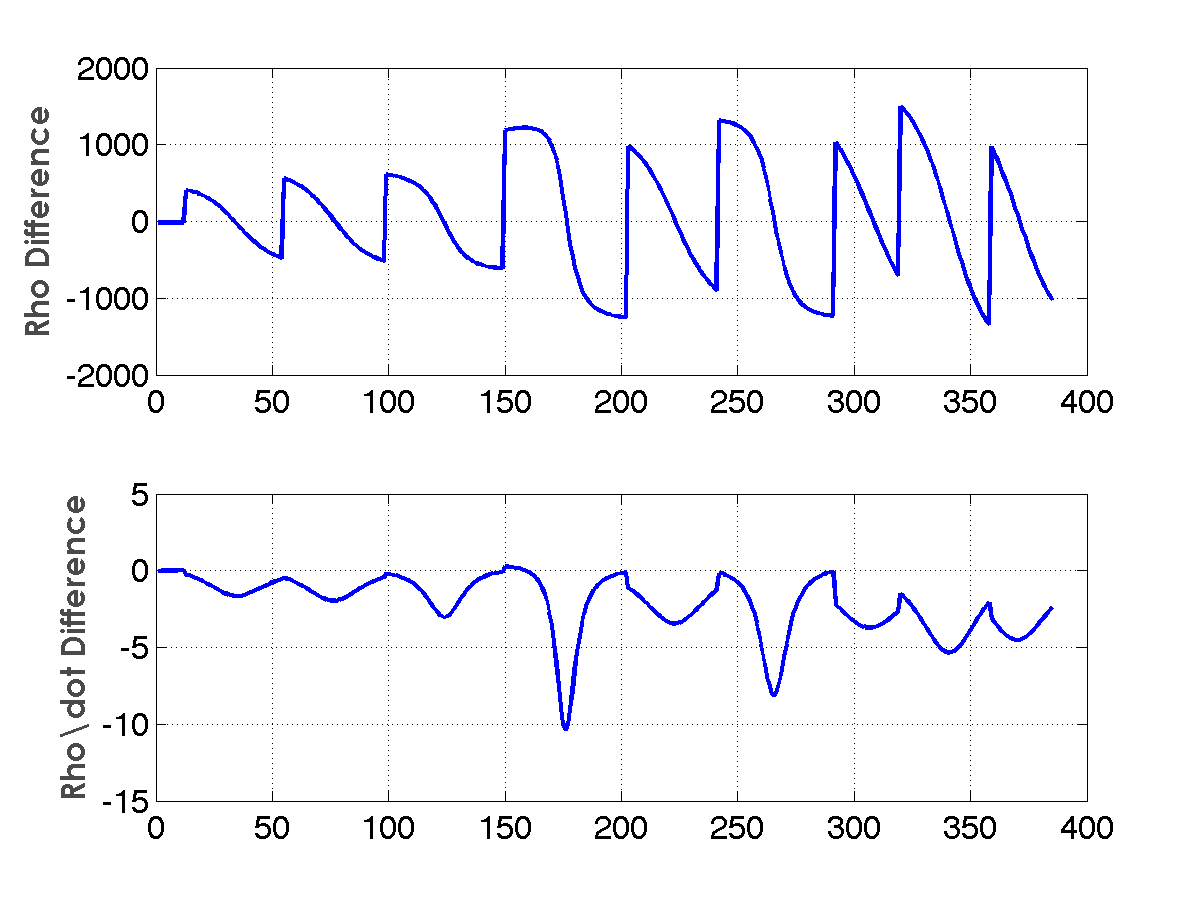
\includegraphics[scale=0.75]{1.png}
\end{figure}

Again, these plots look very much like those provided in the solutions, so I consider them verified. 

Finally, I took the RMS of each residual, using the following equation

% 15
\begin{equation}\label{rms}
	rms= \sqrt{\frac{\sum{(\rho_{observed}-\rho_{computed}})^2}{n}}
\end{equation}

Yielding a final rms computation to be:

\begin{displaymath}
	\boxed{ \Large
	\left[ \begin{array}{c}
		\rho_{rms}			\\
		\dot{\rho}_{rms}		\\
	\end{array} \right]
	=
	\left[ \begin{array}{c}
		732.74831			\\
		2.90017				\\
	\end{array}\right]}
\end{displaymath}




%>>>>>>>>>>>>>>>>>>>>>>>>>>>>>>Appendix A<<<<<<<<<<<<<<<<<<<<<<<<<<<<<<<<


\vspace{8in}
\appendix{\centerline{\LARGE \bf{Appendix A - MATLAB Code}}}

\begin{lstlisting}
%%%%%%%%%%%%%%%%%%%%%%%%%%%%%%%%%%%%%%%%%%%%%%%%%%%%%%%%%%%%%%%%%%%%%%%%
% 
% 
% Zach Dischner-10/21/2012
% 
% ASEN 5070-Statistical Orbit Determination
% 
% Homework 7
% 
% 
%%%%%%%%%%%%%%%%%%%%%%%%%%%%%%%%%%%%%%%%%%%%%%%%%%%%%%%%%%%%%%%%%%%%%%%%

clc;clear all;close all; format compact;format long g;tic



%% 1 - Derive A_18x18 and Htilde_2x18

% [A,Htilde]= FindA_Htilde();
% fprintf('A and Htilde were found. Not shown since they are too big to glean any insight from')

%% 2 - Perform integration
%--------------------------------------------- 
%Constants
tol = 1e-13;
uE  = 3.986004415e14;               % m^3/s^2
J2  = 0.00108248;                   % []
Cd  = 2;
theta_dot  = 7.29211585530066e-5;   % rad/s
%--------------------------------------------- 


%--------------------------------------------- 
%Initial Conditions
time    = [0:20:18340];

RV_Init         = [757700,5222607.0,4851500.0,2213.21,4678.34,-5371.30];
Station_Init    = [-5127510.0 , -3794160.0 , 0.0 ,...               %101
                    3860910.0  , 3238490.0  , 3898094.0 , ...       %337
                    549505.0 , -1380872.0 , 6182197.0 ];            %394
Const_Init = [uE , J2 , Cd ];

Phi_Init = eye(18);
StateInit = [RV_Init , Const_Init , Station_Init , reshape(Phi_Init,1,length(Phi_Init)^2)]';
%--------------------------------------------- 


%--------------------------------------------- 
% Integrate
tol_mat = ones(size(StateInit)) .* tol;
options = odeset('RelTol',tol,'AbsTol',tol_mat,'OutputFcn',@odetpbar);

% ode_options = odeset('RelTol',1e-13,'AbsTol',1e-13,'OutputFcn',@odetpbar);

[time,StatePhi] = ode45('StateDeriv_WithPhi',time,StateInit,options);

for ii = 1:length(time)
       Phi{ii} = reshape(StatePhi(ii,19:end),size(Phi_Init));
       State(ii,:) = StatePhi(ii,1:18);
end
%---------------------------------------------

fprintf('State(18340,0)  ==>   %f3.5 \n\n',State(time(end)/20,1))


%% 3 - Compare Residules of Observed and Computed Range and Range Rate 
%--------------------------------------------- 
%Rho and Rho dot equations (Turn into Wences' awesome function)
rho = @(x,y,z,Xsite,Ysite,Zsite,theta) sqrt(x^2+y^2+z^2+Xsite^2+Ysite^2+Zsite^2-2*(x*Xsite+y*Ysite)*cos(theta)+2*(x*Ysite-y*Xsite)*sin(theta)-2*z*Zsite);
rhodot = @(x,y,z,xdot,ydot,zdot,Xsite,Ysite,Zsite,theta,theta_dot,rho) (x*xdot + y*ydot + z*zdot - (xdot*Xsite + ydot*Ysite)*cos(theta) + theta_dot*(x*Xsite + y*Ysite)*sin(theta)...
            +(xdot*Ysite - ydot*Xsite)*sin(theta) + theta_dot*(x*Ysite - y*Xsite)*cos(theta) - zdot*Zsite)...
                                                                    /rho;
%---------------------------------------------                                                                 
            

%---------------------------------------------                                                            
% Load in Observation Data
obs         = load('Observations.mat');
time_obs    = obs.obs(:,1);
station     = obs.obs(:,2);
rho_obs     = obs.obs(:,3);
rhodot_obs  = obs.obs(:,4);
%---------------------------------------------


SatState = cell(18,1);
rho_comp = zeros(length(time_obs),1); rhodot_comp = rho_comp;

%--------------------------------------------- 
% Generate rho, rhodot  ==> G
for ii = 1:length(time_obs);
    
    index = time == time_obs(ii);
    SatState=num2cell(State(index,:));
    
    
    [x,y,z,xdot,ydot,zdot,uE,J2,Cd,Xsite1,Ysite1,Zsite1,Xsite2,Ysite2,Zsite2,Xsite3,Ysite3,Zsite3] = SatState{:};
    
    %Station 1
    if station(ii) == 101
        Xsite=Xsite1;   Ysite=Ysite1;   Zsite=Zsite1;
    end
    
    %Station 2
    if station(ii) == 337
        Xsite=Xsite2;   Ysite=Ysite2;   Zsite=Zsite2;
    end
    
    %Station 3
    if station(ii) == 394
        Xsite=Xsite3;   Ysite=Ysite3;   Zsite=Zsite3;
    end
    
    
    theta = (time_obs(ii)*theta_dot);
    rho_comp(ii)    = rho(x,y,z,Xsite,Ysite,Zsite,theta);
    rhodot_comp(ii) = rhodot(x,y,z,xdot,ydot,zdot,Xsite,Ysite,Zsite,theta,theta_dot,rho_comp(ii));
    G(ii,:) = [rho_comp(ii),rhodot_comp(ii)];
end
%--------------------------------------------- 


%--------------------------------------------- 
% Display Results
rho_diff = (rho_obs - rho_comp);
rhodot_diff = (rhodot_obs - rhodot_comp);
subplot(2,1,1)
plot(rho_diff)
ylabel('Rho Difference')
subplot(2,1,2)
plot(rhodot_diff)
ylabel('Rho Difference')

range_rms = sqrt(sum(rho_diff.^2)/length(rho_diff));
range_rate_rms = sqrt(sum(rhodot_diff.^2)/length(rhodot_diff));

fprintf('Range RMS is  ==>  %3.5f\n',range_rms)
fprintf('Range Rate RMS is  ==>  %3.5f\n\n',range_rate_rms)
%--------------------------------------------- 



fprintf('Time it took to run is : %f3.5',toc)

figure_awesome('save')






function [A Htilde] = FindA_Htilde()

%%%%%%%%%%%%%%%%%%%%%%%%%%%%%%%%%%%%%%%%%%%%%%%%%%%%%%%%%%%%%%%%%%%%%%%%
% 
% 
% Zach Dischner-10/21/2012
% 
% FindA_Htilde
% 
% Purpose: Find A and Htilde matrices
% 
% 
%%%%%%%%%%%%%%%%%%%%%%%%%%%%%%%%%%%%%%%%%%%%%%%%%%%%%%%%%%%%%%%%%%%%%%%%






% Use Jacobian

%% Define the State
syms x y z xdot ydot zdot uE J2 Cd Xsite1  Ysite1  Zsite1 Xsite2 Ysite2 Zsite2  Xsite3 Ysite3 Zsite3 theta theta_dot
syms R_E r Area m rho_a Va va 

X       = [x ; y ; z ; xdot ; ydot ; zdot ; uE ; J2 ; Cd ; Xsite1 ; Ysite1 ; Zsite1; Xsite2; Ysite2; Zsite2 ; Xsite3; Ysite3; Zsite3];

%% Define F vector

% [xdot ydot zdot] due to gravity and J2
r       = sqrt(x^2+y^2+z^2);
F_U     = [...
              -uE/r^3*x*(1-3/2*J2*(R_E/r)^2*(5*(z/r)^2-1));
              -uE/r^3*y*(1-3/2*J2*(R_E/r)^2*(5*(z/r)^2-1));
              -uE/r^3*z*(1-3/2*J2*(R_E/r)^2*(5*(z/r)^2-3));
          ];
      
% [xdot ydot zdot] due to atmospheric drag
Va      = [
    xdot + theta_dot*y;
    ydot - theta_dot*x;
    zdot
    ];
va      = sqrt((xdot + theta_dot*y)^2 + (ydot - theta_dot*x)^2 + zdot^2);

syms rho0 r0 H
rho_a   = rho0.*exp((r - r0)./H);

F_Drag = -0.5 .* Cd .* (Area./m) .* rho_a .* va .* Va;

% Assemble
F_a = F_U + F_Drag; % 

% X' = F*X
F =[xdot ; ydot ; zdot ; F_a ; 0 ; 0 ; 0 ; 0 ; 0 ; 0 ; 0 ; 0 ; 0 ; 0 ; 0 ; 0];
      

%% Find A Matrix
clear r; syms r
A = jacobian(F,X);
% Do this outside of the function?
A=simplify(A);
A=subs(A,sqrt(x^2+y^2+z^2),r);
A=subs(A,(x^2+y^2+z^2),r^2);
A = simplify(A);

matlabFunction(A,'file','A_18x18.m')



%% Find Htilde Matrix (for a generic station position)
syms Xsite Ysite Zsite
syms theta  % = theta_dot * time
% dcm = [cos -sin 0;sin cos 0; 0 0 1];
% rho = sqrt((x-Xsite*cos(theta) - Ysite*sin(theta))^2 + (y-Ysite*cos(theta) + Xsite*sin(theta))^2 + (z-Zsite)^2);
% The Answer
rho = sqrt(x^2+y^2+z^2+Xsite^2+Ysite^2+Zsite^2+2*(x*Xsite+y*Ysite)*cos(theta)+2*(x*Ysite-y*Xsite)*sin(theta)-2*z*Zsite);
% rho = @(x,y,z,Xsite,Ysite,Zsite,theta) sqrt(x^2+y^2+z^2+Xsite^2+Ysite^2+Zsite^2+2*(x*Xsite+y*Ysite)*cos(theta)+2*(x*Ysite-y*Xsite)*sin(theta)-2*z*Zsite)

rhodot = (x*xdot + y*ydot + z*zdot - (xdot*Xsite + ydot*Ysite)*cos(theta) + theta_dot*(x*Xsite + y*Ysite)*sin(theta)...
            +(xdot*Ysite - ydot*Xsite)*sin(theta) + theta_dot*(x*Ysite - y*Xsite)*cos(theta) - zdot*Zsite)...
                                                            /rho;
obs = [rho;rhodot];

% For just single station
Single_Station_X       = [x ; y ; z ; xdot ; ydot ; zdot ; uE ; J2 ; Cd ; Xsite ; Ysite ; Zsite];

% Add padding depending on the station. 
% If station 1, add 6 columns of padding
% If station 2, add 3 columns, move 3 endmost columns after that, then add
% 3 columns
% IF station 3, put 6 columns of zeros between the 9th and (going to 15th) columms. 

Htilde = jacobian(obs,Single_Station_X);

matlabFunction(Htilde,'file','Htilde_2x12.m')



end



function Xprime = StateDeriv_WithPhi(time,X)
%
%Author: 
%           Zach Dischner
%Date:
%           10/18/2012
%Use: 
%           StateHistory=ode45(StateDeriv_WithPhi,[linspace(1,100),X_init)
% 
% Derivative function, designed to return the derivative of the Cartesian
%   R and V observations, incliuding the effect of the Earth's Oblateness
%   and drag. In addition, return the PHI matrix, reformed into a single
%   vector. 
%
% Written by Zach Dischner on 8/30/2012
%
% inputs:
%         time: time...
%         State  : A column vector. 18-state + PHI reformed
%                       X
%                       Y
%                       Z
%                       X'
%                       Y'
%                       Z'
%                       u_e
%                       J2
%                       Cd
%                       Xbar_sitei   (1 2 or 3) based on station coordinates
%                       Phi
%
%

%% Define Constants
% Oblateness
uE   = 3.986004415e14;                     % m^3/s^2
J2   = 1.082626925638815e-3;                % []
R_E  = 6378136.3;                           % m    Radius of earth

% Drag
Cd      = 2.0;
Area    = 3.0;                  % m^2
m       = 970;                  % kg
rho0    = 3.614e-13;            % kg/m^3
r0      = 700000.0 + R_E;       % m
H       = 88667.0;              % m
theta_dot  = 7.29211585530066e-5;  % rad/s




%% Form State Variables
Phi=reshape(X(19:end),sqrt(length(X(19:end))),sqrt(length(X(19:end))));
% Type this out for speed later
SatState = cell(18,1);
SatState=num2cell(X(1:18));
[x,y,z,xdot,ydot,zdot,na,na1,na2, ...
    Xsite1,Ysite1,Zsite1,Xsite2,Ysite2,Zsite2 ...
    Xsite3,Ysite3,Zsite3] = SatState{:};

r=sqrt(x^2 + y^2 + z^2);

%% Use Force Equations
F_U     = [...
              -uE/r^3*x*(1-3/2*J2*(R_E/r)^2*(5*(z/r)^2-1));
              -uE/r^3*y*(1-3/2*J2*(R_E/r)^2*(5*(z/r)^2-1));
              -uE/r^3*z*(1-3/2*J2*(R_E/r)^2*(5*(z/r)^2-3));
          ];
      
% [xdot ydot zdot] due to atmospheric drag
Va      = [
    xdot + theta_dot*y;
    ydot - theta_dot*x;
    zdot
    ];
va      = sqrt((xdot + theta_dot*y)^2 + (ydot - theta_dot*x)^2 + zdot^2);

rho_a   = rho0.*exp(-(r - r0)./H);

F_Drag = -0.5 .* Cd .* (Area./m) .* rho_a .* va .* Va;

% Assemble
F_a = F_U + F_Drag;

State_Deriv = [xdot ; ydot ; zdot ; F_a ; 0 ; 0 ; 0 ; 0 ; 0 ; 0 ; 0 ; 0 ; 0 ; 0 ; 0 ; 0]; % Add in station location with earth's rotation rate

% For now 
% A=load('A.mat');



%% Integrate Phi
 A = A_18x18(Area,Cd,H,J2,R_E,m,r,r0,rho0,theta_dot,uE,x,xdot,y,ydot,z,zdot);
                                                                                                                                                                                                                                                                                                                                                                                                                                                                                                                                                          

bounds = length(Phi);
PhiPrime = A(1:bounds,1:bounds)*Phi;


%% Reform full state vector
Xprime = [State_Deriv ; reshape(PhiPrime,length(PhiPrime)^2,1)];

end

\end{lstlisting}




%>>>>>>>>>>>>>>>>>>>>>>>>>>>>>>Appendix B<<<<<<<<<<<<<<<<<<<<<<<<<<<<<<<<


\vspace{8in}
\appendix{\centerline{\LARGE \bf{Appendix B - MATLAB Generation Code}}}


% This LaTeX was auto-generated from an M-file by MATLAB.
% To make changes, update the M-file and republish this document.




\sloppy
\definecolor{lightgray}{gray}{0.5}
\setlength{\parindent}{0pt}



    
    
\subsection*{Contents}

\begin{itemize}
\setlength{\itemsep}{-1ex}
   \item 1 - Derive A\_18x18 and Htilde\_2x18
   \item 2 - Perform integration
   \item 3 - Compare Residules of Observed and Computed Range and Range Rate
\end{itemize}
\begin{verbatim}
%%%%%%%%%%%%%%%%%%%%%%%%%%%%%%%%%%%%%%%%%%%%%%%%%%%%%%%%%%%%%%%%%%%%%%%%
%
%
% Zach Dischner-10/21/2012
%
% ASEN 5070-Statistical Orbit Determination
%
% Homework 7
%
%
%%%%%%%%%%%%%%%%%%%%%%%%%%%%%%%%%%%%%%%%%%%%%%%%%%%%%%%%%%%%%%%%%%%%%%%%

clc;clear all;close all; format compact;format long g;tic
\end{verbatim}


\subsection*{1 - Derive A\_18x18 and Htilde\_2x18}

\begin{verbatim}
% [A,Htilde]= FindA_Htilde();
% fprintf('A and Htilde were found. Not shown since they are too big to glean any insight from')
\end{verbatim}


\subsection*{2 - Perform integration}

\begin{verbatim}
%---------------------------------------------
%Constants
tol = 1e-13;
uE  = 3.986004415e14;               % m^3/s^2
J2  = 0.00108248;                   % []
Cd  = 2;
theta_dot  = 7.29211585530066e-5;   % rad/s
%---------------------------------------------


%---------------------------------------------
%Initial Conditions
time    = [0:20:18340];

RV_Init         = [757700,5222607.0,4851500.0,2213.21,4678.34,-5371.30];
Station_Init    = [-5127510.0 , -3794160.0 , 0.0 ,...               %101
                    3860910.0  , 3238490.0  , 3898094.0 , ...       %337
                    549505.0 , -1380872.0 , 6182197.0 ];            %394
Const_Init = [uE , J2 , Cd ];

Phi_Init = eye(18);
StateInit = [RV_Init , Const_Init , Station_Init , reshape(Phi_Init,1,length(Phi_Init)^2)]';
%---------------------------------------------


%---------------------------------------------
% Integrate
tol_mat = ones(size(StateInit)) .* tol;
options = odeset('RelTol',tol,'AbsTol',tol_mat,'OutputFcn',@odetpbar);

% ode_options = odeset('RelTol',1e-13,'AbsTol',1e-13,'OutputFcn',@odetpbar);

[time,StatePhi] = ode45('StateDeriv_WithPhi',time,StateInit,options);

for ii = 1:length(time)
       Phi{ii} = reshape(StatePhi(ii,19:end),size(Phi_Init));
       State(ii,:) = StatePhi(ii,1:18);
end
%---------------------------------------------

fprintf('State(18340,0)  ==>   %f3.5 \n\n',State(time(end)/20,1))
\end{verbatim}

        \color{lightgray} \begin{verbatim}ODE integration: 100%    [..........]
   Integration time: 6.0819
State(18340,0)  ==>   1088759.4876233.5 

\end{verbatim} \color{black}
    

\subsection*{3 - Compare Residules of Observed and Computed Range and Range Rate}

\begin{verbatim}
%---------------------------------------------
%Rho and Rho dot equations (Turn into Wences' awesome function)
rho = @(x,y,z,Xsite,Ysite,Zsite,theta) sqrt(x^2+y^2+z^2+Xsite^2+Ysite^2+Zsite^2-2*(x*Xsite+y*Ysite)*cos(theta)+2*(x*Ysite-y*Xsite)*sin(theta)-2*z*Zsite);
rhodot = @(x,y,z,xdot,ydot,zdot,Xsite,Ysite,Zsite,theta,theta_dot,rho) (x*xdot + y*ydot + z*zdot - (xdot*Xsite + ydot*Ysite)*cos(theta) + theta_dot*(x*Xsite + y*Ysite)*sin(theta)...
            +(xdot*Ysite - ydot*Xsite)*sin(theta) + theta_dot*(x*Ysite - y*Xsite)*cos(theta) - zdot*Zsite)...
                                                                    /rho;
%---------------------------------------------


%---------------------------------------------
% Load in Observation Data
obs         = load('Observations.mat');
time_obs    = obs.obs(:,1);
station     = obs.obs(:,2);
rho_obs     = obs.obs(:,3);
rhodot_obs  = obs.obs(:,4);
%---------------------------------------------


SatState = cell(18,1);
rho_comp = zeros(length(time_obs),1); rhodot_comp = rho_comp;

%---------------------------------------------
% Generate rho, rhodot  ==> G
for ii = 1:length(time_obs);

    index = time == time_obs(ii);
    SatState=num2cell(State(index,:));


    [x,y,z,xdot,ydot,zdot,uE,J2,Cd,Xsite1,Ysite1,Zsite1,Xsite2,Ysite2,Zsite2,Xsite3,Ysite3,Zsite3] = SatState{:};

    %Station 1
    if station(ii) == 101
        Xsite=Xsite1;   Ysite=Ysite1;   Zsite=Zsite1;
    end

    %Station 2
    if station(ii) == 337
        Xsite=Xsite2;   Ysite=Ysite2;   Zsite=Zsite2;
    end

    %Station 3
    if station(ii) == 394
        Xsite=Xsite3;   Ysite=Ysite3;   Zsite=Zsite3;
    end


    theta = (time_obs(ii)*theta_dot);
    rho_comp(ii)    = rho(x,y,z,Xsite,Ysite,Zsite,theta);
    rhodot_comp(ii) = rhodot(x,y,z,xdot,ydot,zdot,Xsite,Ysite,Zsite,theta,theta_dot,rho_comp(ii));
    G(ii,:) = [rho_comp(ii),rhodot_comp(ii)];
end
%---------------------------------------------


%---------------------------------------------
% Display Results
rho_diff = (rho_obs - rho_comp);
rhodot_diff = (rhodot_obs - rhodot_comp);
subplot(2,1,1)
plot(rho_diff)
ylabel('Rho Difference')
subplot(2,1,2)
plot(rhodot_diff)
ylabel('Rho\dot Difference')

range_rms = sqrt(sum(rho_diff.^2)/length(rho_diff));
range_rate_rms = sqrt(sum(rhodot_diff.^2)/length(rhodot_diff));

fprintf('Range RMS is  ==>  %3.5f\n',range_rms)
fprintf('Range Rate RMS is  ==>  %3.5f\n\n',range_rate_rms)
%---------------------------------------------

fprintf('Time it took to run is : %f3.5',toc)

figure_awesome('save')
\end{verbatim}

        \color{lightgray} \begin{verbatim}Range RMS is  ==>  732.74831
Range Rate RMS is  ==>  2.90017

Time it took to run is : 8.1296113.5Warning: Unable to interpret TeX string "Rho\dot Difference" 
\end{verbatim} \color{black}
    

    








\end{document}